\documentclass[tikz]{standalone}
\usetikzlibrary{shapes.callouts}
\tikzset{
    level/.style = {
        ultra thick,
        black,
    },
    connect/.style = {
        dashed,
        black
    },
    notice/.style = {
        draw,
        rectangle callout,
        callout relative pointer={#1}
    },
    label/.style = {
        text width=2cm
    }
}
\begin{document}
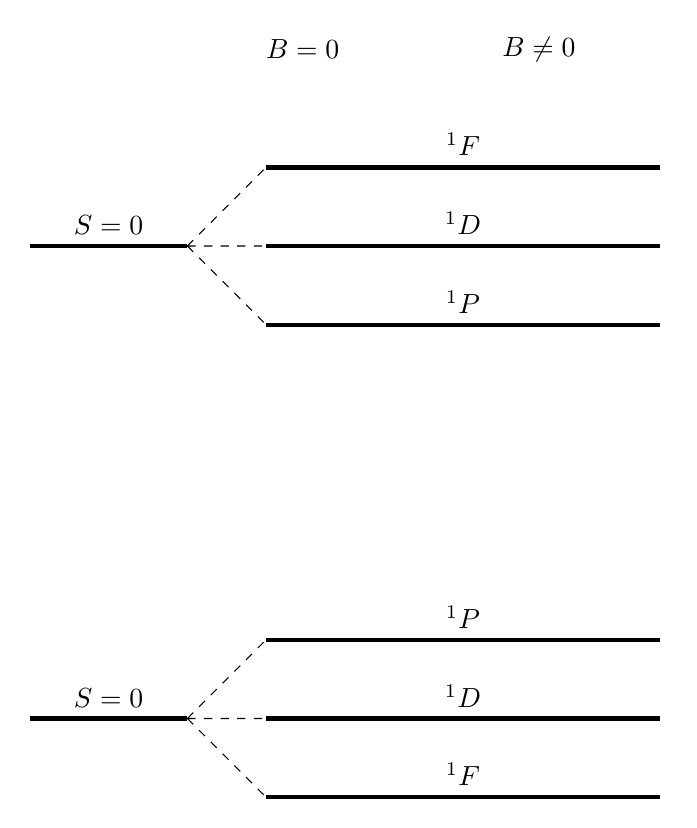
\begin{tikzpicture}
    % Draw all levels
    \draw[level] (0,+3)  -- node[above] {$S=0$} (2,+3);
    \draw[level] (0,-3)  -- node[above] {$S=0$} (2,-3);

    \draw[connect] (2,+3) -- (3,+4) (2,+3) -- (3,+3) (2,+3) -- (3,+2);
    \draw[connect] (2,-3) -- (3,-4) (2,-3) -- (3,-3) (2,-3) -- (3,-2);

    \draw[level] (3,+2) -- node[above] {$^1P$} (8,+2);
    \draw[level] (3,+3) -- node[above] {$^1D$} (8,+3);
    \draw[level] (3,+4) -- node[above] {$^1F$} (8,+4);
    \draw[level] (3,-2) -- node[above] {$^1P$} (8,-2);
    \draw[level] (3,-3) -- node[above] {$^1D$} (8,-3);
    \draw[level] (3,-4) -- node[above] {$^1F$} (8,-4);

    % Draw labels
    \node[label] at (4,5.5) {$B = 0$};
    \node[label] at (7,5.5) {$B \neq 0$};
\end{tikzpicture}
\end{document}
